\documentclass[convert={density=600,size=672x480,outext=.png}]{standalone}
\usepackage{tikz}
\usetikzlibrary{calc, shapes, positioning, decorations.text, arrows.meta,
                trees,positioning,arrows,chains,shapes.geometric,automata,%
                decorations.pathreplacing,decorations.pathmorphing,shapes,%
                matrix,shapes.symbols,plotmarks,decorations.markings,shadows}
\usepackage{tikzscale}
\usepackage{pgfplots}

\definecolor{mybluetikz}{RGB}{86,180,233}
\definecolor{myredtikz}{RGB}{213,94,0}
\definecolor{mygreen}{RGB}{124,174,0}

\definecolor[named]{myblue}{RGB}{0,102,204}
\definecolor[named]{myred}{RGB}{174,49,54}

%%%%%%%%%%%%%%%%%%%%%%%%%%%%%%%%%%%%%%%%%%%%%%%%%
%
% Some definitions for TikZ graphics
%
%%%%%%%%%%%%%%%%%%%%%%%%%%%%%%%%%%%%%%%%%%%%%%%%%

\tikzset{
  root/.style = {rectangle,rounded corners, text width=7em, text centered, inner sep=2mm,
                 align = center, top color=white,
                 bottom color=blue!50!black!20, draw=blue!40!black!60, very thick},
  goodnode/.style = {rectangle, rounded corners, text width = 7em, text centered, inner sep = 2mm,
                     draw = mygreen!60,
                     top color = white, bottom color = mygreen!40, very thick},
  badnode/.style = {rectangle, rounded corners,text width = 7em, text centered, inner sep = 2mm,
                    draw = myredtikz!60,
                    top color = white, bottom color = myredtikz!40, very thick},
  nonode/.style = {rectangle, rounded corners, text width = 7em, text centered, inner sep = 2mm,
                   draw = mybluetikz!60,
                   top color = white, bottom color = mybluetikz!40, very thick}
}

\pgfplotsset{compat = 1.12,
     cmhplot/.style={color=mybluetikz,mark=none,line width=3pt,-},
     cmhplotouter/.style={color=mybluetikz!70,mark=none,line width=3pt,-},
     cmhplotobs/.style={color=mybluetikz,mark=none,line width=2pt,-},
     cmhplotbuys/.style={color=mygreen!40,mark=none,line width=1.5pt,-},
     cmhplotsells/.style={color=myredtikz!40,mark=none,line width=1.5pt,-},
     soldot/.style={color=myredtikz,only marks,mark=*, mark size = 3.5},
     holdot/.style={color=myredtikz,fill=white,only marks,mark=*, mark size = 3.5},
     soldotouter/.style={color=myredtikz!70,only marks,mark=*, mark size = 3.5},
     holdotouter/.style={color=myredtikz!70,fill=white,only marks,mark=*, mark size = 3.5},
     soldotbuys/.style={color=mygreen!40,only marks,mark=*, mark size = 2},
     holdotbuys/.style={color=mygreen!40,fill=white,only marks,mark=*, mark size = 2},
     holdotbuysreset/.style={color=mygreen!40,fill=white,only marks,mark=square*, mark size = 3},
     soldotsells/.style={color=myredtikz!40,only marks,mark=*, mark size = 2},
     holdotsells/.style={color=myredtikz!40,fill=white,only marks,mark=*, mark size = 2},
     holdotsellsreset/.style={color=myredtikz!40,fill=white,only marks,mark=square*, mark size = 3},
     soldotobs/.style={color=mybluetikz,only marks,mark=*, mark size = 2.5},
     holdotobs/.style={color=mybluetikz,fill=white,only marks,mark=*, mark size = 2.5},
}
\begin{document}
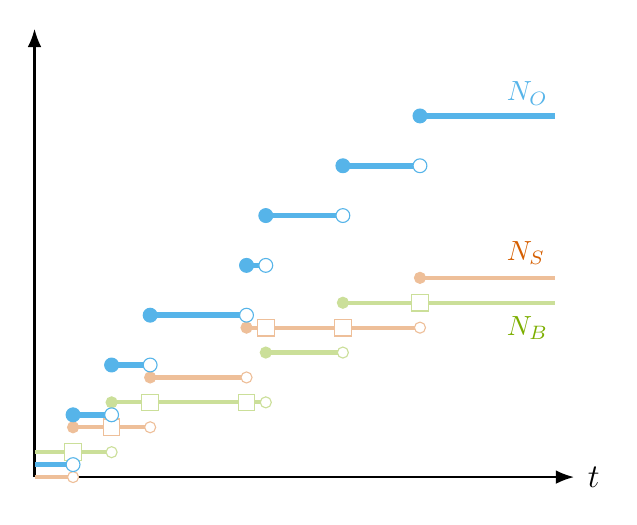
\begin{tikzpicture}
% \pgfmathsetlengthmacro\MajorTickLength{
%     \pgfkeysvalueof{/pgfplots/major tick length} * 1.5
%   }
    \begin{axis}[
            axis x line = bottom,
            axis y line = left,
            xlabel = {\large $t$},
            ylabel = {},
            ytick = \empty,
            xtick = \empty,
            %xticklabels = {0,$\originmarket$, $\closemarket$},
            axis line style={-Latex, thick},
            xmin=0,xmax=7,
            ymin=0,ymax=9,
            every axis x label/.style={
            at={(ticklabel* cs:1.0075)},
            anchor=west,
            },
            % every axis y label/.style={
            % at={(ticklabel* cs:1.0075)},
            % anchor=south,
            % },
            % thick,
            clip=false,
            % major tick length=\MajorTickLength,
            % every tick/.style={
            % black,
            % very thick}
        ]
        \addplot[cmhplotbuys,-,domain=0:1]{0.5};
        \addplot[cmhplotbuys,-,domain=1:3]{1.5};
        \addplot[cmhplotbuys,-,domain=3:4]{2.5};
        \addplot[cmhplotbuys,-,domain=4:6.75]{3.5};
        %
        \addplot[cmhplotsells,-,domain=0:0.5]{0};
        \addplot[cmhplotsells,-,domain=0.5:1.5]{1};
        \addplot[cmhplotsells,-,domain=1.5:2.75]{2};
        \addplot[cmhplotsells,-,domain=2.75:5]{3};
        \addplot[cmhplotsells,-,domain=5:6.75]{4};
        %
        \addplot[cmhplotobs,-,domain=0:0.5]{0.25};
        \addplot[cmhplotobs,-,domain=0.5:1]{1.25};
        \addplot[cmhplotobs,-,domain=1:1.5]{2.25};
        \addplot[cmhplotobs,-,domain=1.5:2.75]{3.25};
        \addplot[cmhplotobs,-,domain=2.75:3]{4.25};
        \addplot[cmhplotobs,-,domain=3:4]{5.25};
        \addplot[cmhplotobs,-,domain=4:5]{6.25};
        \addplot[cmhplotobs,-,domain=5:6.75]{7.25};
        %
        \addplot[holdotbuys]coordinates{(1,0.5)(3,1.5)(4,2.5)(5,3.5)};
        \addplot[soldotbuys]coordinates{(1,1.5)(3,2.5)(4,3.5)};
        \addplot[holdotbuysreset]coordinates{(0.5,0.5)(1.5,1.5)(2.75,1.5)(5,3.5)};
        %
        \addplot[holdotsells]coordinates{(0.5,0)(1.5,1)(2.75,2)(5,3)};
        \addplot[soldotsells]coordinates{(0.5,1)(1.5,2)(2.75,3)(5,4)};
        \addplot[holdotsellsreset]coordinates{(1,1)(3,3)(4,3)};
        %
        \addplot[holdotobs]coordinates{(0.5,0.25)(1,1.25)(1.5,2.25)(2.75,3.25)(3,4.25)(4,5.25)(5,6.25)};
        \addplot[soldotobs]coordinates{(0.5,1.25)(1,2.25)(1.5,3.25)(2.75,4.25)(3,5.25)(4,6.25)(5,7.25)};
        \node[anchor=west, text = myredtikz, align = center] (source) at (axis cs:6,4.5){$N_S$};
        \node[anchor=west, text = mygreen, align = center] (source) at (axis cs:6,3){$N_B$};
        \node[anchor=west, text = mybluetikz, align = center] (source) at (axis cs:6,7.7){$N_O$};
    \end{axis}
\end{tikzpicture}
\end{document}